\documentclass[]{tufte-handout}

% ams
\usepackage{amssymb,amsmath}

\usepackage{ifxetex,ifluatex}
\usepackage{fixltx2e} % provides \textsubscript
\ifnum 0\ifxetex 1\fi\ifluatex 1\fi=0 % if pdftex
  \usepackage[T1]{fontenc}
  \usepackage[utf8]{inputenc}
\else % if luatex or xelatex
  \makeatletter
  \@ifpackageloaded{fontspec}{}{\usepackage{fontspec}}
  \makeatother
  \defaultfontfeatures{Ligatures=TeX,Scale=MatchLowercase}
  \makeatletter
  \@ifpackageloaded{soul}{
     \renewcommand\allcapsspacing[1]{{\addfontfeature{LetterSpace=15}#1}}
     \renewcommand\smallcapsspacing[1]{{\addfontfeature{LetterSpace=10}#1}}
   }{}
  \makeatother

\fi

% graphix
\usepackage{graphicx}
\setkeys{Gin}{width=\linewidth,totalheight=\textheight,keepaspectratio}

% booktabs
\usepackage{booktabs}

% url
\usepackage{url}

% hyperref
\usepackage{hyperref}

% units.
\usepackage{units}


\setcounter{secnumdepth}{-1}

% citations
\usepackage{natbib}
\bibliographystyle{plainnat}

% pandoc syntax highlighting
\usepackage{color}
\usepackage{fancyvrb}
\newcommand{\VerbBar}{|}
\newcommand{\VERB}{\Verb[commandchars=\\\{\}]}
\DefineVerbatimEnvironment{Highlighting}{Verbatim}{commandchars=\\\{\}}
% Add ',fontsize=\small' for more characters per line
\newenvironment{Shaded}{}{}
\newcommand{\AlertTok}[1]{\textcolor[rgb]{1.00,0.00,0.00}{\textbf{#1}}}
\newcommand{\AnnotationTok}[1]{\textcolor[rgb]{0.38,0.63,0.69}{\textbf{\textit{#1}}}}
\newcommand{\AttributeTok}[1]{\textcolor[rgb]{0.49,0.56,0.16}{#1}}
\newcommand{\BaseNTok}[1]{\textcolor[rgb]{0.25,0.63,0.44}{#1}}
\newcommand{\BuiltInTok}[1]{#1}
\newcommand{\CharTok}[1]{\textcolor[rgb]{0.25,0.44,0.63}{#1}}
\newcommand{\CommentTok}[1]{\textcolor[rgb]{0.38,0.63,0.69}{\textit{#1}}}
\newcommand{\CommentVarTok}[1]{\textcolor[rgb]{0.38,0.63,0.69}{\textbf{\textit{#1}}}}
\newcommand{\ConstantTok}[1]{\textcolor[rgb]{0.53,0.00,0.00}{#1}}
\newcommand{\ControlFlowTok}[1]{\textcolor[rgb]{0.00,0.44,0.13}{\textbf{#1}}}
\newcommand{\DataTypeTok}[1]{\textcolor[rgb]{0.56,0.13,0.00}{#1}}
\newcommand{\DecValTok}[1]{\textcolor[rgb]{0.25,0.63,0.44}{#1}}
\newcommand{\DocumentationTok}[1]{\textcolor[rgb]{0.73,0.13,0.13}{\textit{#1}}}
\newcommand{\ErrorTok}[1]{\textcolor[rgb]{1.00,0.00,0.00}{\textbf{#1}}}
\newcommand{\ExtensionTok}[1]{#1}
\newcommand{\FloatTok}[1]{\textcolor[rgb]{0.25,0.63,0.44}{#1}}
\newcommand{\FunctionTok}[1]{\textcolor[rgb]{0.02,0.16,0.49}{#1}}
\newcommand{\ImportTok}[1]{#1}
\newcommand{\InformationTok}[1]{\textcolor[rgb]{0.38,0.63,0.69}{\textbf{\textit{#1}}}}
\newcommand{\KeywordTok}[1]{\textcolor[rgb]{0.00,0.44,0.13}{\textbf{#1}}}
\newcommand{\NormalTok}[1]{#1}
\newcommand{\OperatorTok}[1]{\textcolor[rgb]{0.40,0.40,0.40}{#1}}
\newcommand{\OtherTok}[1]{\textcolor[rgb]{0.00,0.44,0.13}{#1}}
\newcommand{\PreprocessorTok}[1]{\textcolor[rgb]{0.74,0.48,0.00}{#1}}
\newcommand{\RegionMarkerTok}[1]{#1}
\newcommand{\SpecialCharTok}[1]{\textcolor[rgb]{0.25,0.44,0.63}{#1}}
\newcommand{\SpecialStringTok}[1]{\textcolor[rgb]{0.73,0.40,0.53}{#1}}
\newcommand{\StringTok}[1]{\textcolor[rgb]{0.25,0.44,0.63}{#1}}
\newcommand{\VariableTok}[1]{\textcolor[rgb]{0.10,0.09,0.49}{#1}}
\newcommand{\VerbatimStringTok}[1]{\textcolor[rgb]{0.25,0.44,0.63}{#1}}
\newcommand{\WarningTok}[1]{\textcolor[rgb]{0.38,0.63,0.69}{\textbf{\textit{#1}}}}

% longtable

% multiplecol
\usepackage{multicol}

% strikeout
\usepackage[normalem]{ulem}

% morefloats
\usepackage{morefloats}


% tightlist macro required by pandoc >= 1.14
\providecommand{\tightlist}{%
  \setlength{\itemsep}{0pt}\setlength{\parskip}{0pt}}

% title / author / date
\title{Try Bayesian Survival Analysis using the JACC study data (Bayesian
Survival Analysis presentations)}
\author{Chaochen Wang \textbar{} Aichi Medical University}
\date{2020-01-12}

\usepackage{booktabs}
\usepackage{longtable}
\usepackage{array}
\usepackage{multirow}
\usepackage{wrapfig}
\usepackage{float}
\usepackage{colortbl}
\usepackage{pdflscape}
\usepackage{tabu}
\usepackage{threeparttable}
\usepackage{threeparttablex}
\usepackage[normalem]{ulem}
\usepackage{makecell}
\usepackage{xcolor}

\begin{document}

\maketitle




\hypertarget{parametric-survival-analysis-model-in-a-bayesian-way}{%
\subsection{Parametric Survival Analysis Model (in a Bayesian
way)}\label{parametric-survival-analysis-model-in-a-bayesian-way}}

\begin{marginfigure}
Weibull Survival funciton in a proportional hazard way expression is:
\[S(t | \mathbf{x}) = \exp\{ -\lambda t ^\kappa e^{\mathbf{\beta_{PH}^T x}} \}\]
\end{marginfigure}

\begin{marginfigure}
Weibull Survival funciton in a AFT way expression is:
\[S(t | \mathbf{x}) = \exp\{ -\lambda t ^\kappa e^{\kappa\mathbf{\beta_{AFT}^T x}} \}\]
\end{marginfigure}

\begin{itemize}
\item
  We chose Weibull model to describe the survival data we have.
\item
  Weibull model is both a proportional hazard model and a accelerated
  failure time (AFT) model. The relationship between the acceleration
  factor and log hazard ratio:
\end{itemize}

\[
\exp(\beta^T_{PH}) = \exp(\kappa\beta^T_{AFT})
\]

\begin{marginfigure}
Acceleration factor is the factor by which time to failure/event is
accelerated for \(x_1 = 1\) compared with \(x_1 = 0\)
\end{marginfigure}

\hypertarget{an-example-of-a-crude-weibull-model-using-the-jags-program-in-r}{%
\subsection{An example of a crude Weibull model using the JAGS program
in
R:}\label{an-example-of-a-crude-weibull-model-using-the-jags-program-in-r}}

\begin{Shaded}
\begin{Highlighting}[]
\NormalTok{jacc.weibull.model <-}\StringTok{ }\ControlFlowTok{function}\NormalTok{() \{}
  \ControlFlowTok{for}\NormalTok{(i }\ControlFlowTok{in} \DecValTok{1}\OperatorTok{:}\DecValTok{39386}\NormalTok{)\{}\CommentTok{# loop through the subjects}
    \CommentTok{# sAge[i] <- (Age[i] - mean(Age[])) / sd(Age[])}
\NormalTok{    is.censored[i] }\OperatorTok{~}\StringTok{ }\KeywordTok{dinterval}\NormalTok{(t[i], c[i])}
\NormalTok{    t[i] }\OperatorTok{~}\StringTok{ }\KeywordTok{dweib}\NormalTok{(shape, lambda[i])}
\NormalTok{    lambda[i] <-}\StringTok{ }\KeywordTok{exp}\NormalTok{(}\OperatorTok{-}\NormalTok{mu[i] }\OperatorTok{*}\StringTok{ }\NormalTok{shape)}
\NormalTok{    mu[i] <-}\StringTok{ }\NormalTok{beta[}\DecValTok{1}\NormalTok{] }\OperatorTok{+}\StringTok{ }\NormalTok{beta[}\DecValTok{2}\NormalTok{]}\OperatorTok{*}\KeywordTok{equals}\NormalTok{(Mlkfre[i], }\DecValTok{2}\NormalTok{) }\OperatorTok{+}
\StringTok{      }\NormalTok{beta[}\DecValTok{3}\NormalTok{]}\OperatorTok{*}\KeywordTok{equals}\NormalTok{(Mlkfre[i], }\DecValTok{3}\NormalTok{) }\OperatorTok{+}\StringTok{ }\NormalTok{beta[}\DecValTok{4}\NormalTok{] }\OperatorTok{*}\StringTok{ }\KeywordTok{equals}\NormalTok{(Mlkfre[i], }\DecValTok{4}\NormalTok{) }\OperatorTok{+}
\StringTok{      }\NormalTok{beta[}\DecValTok{5}\NormalTok{] }\OperatorTok{*}\StringTok{ }\KeywordTok{equals}\NormalTok{(Mlkfre[i], }\DecValTok{5}\NormalTok{) }\CommentTok{# + }
      \CommentTok{# beta[6] * sAge[i]}
    
    \CommentTok{### calculate log-likelihoods}
    \CommentTok{# y[i] <- ifelse(is.censored[i], c[i], t[i])}
    \CommentTok{# loglik[i] <- log(ifelse(is.censored[i],}
    \CommentTok{#                  exp(-lambda[i] * (y[i] ^ shape)),}
    \CommentTok{#               shape * lambda[i] * (y[i] ^ (shape - 1)) * exp(-lambda[i] * (y[i] ^ shape))))}
\NormalTok{  \}}
  
  \CommentTok{## priors for betas}
  \ControlFlowTok{for}\NormalTok{(j }\ControlFlowTok{in} \DecValTok{1}\OperatorTok{:}\DecValTok{5}\NormalTok{)\{}
\NormalTok{    beta[j] }\OperatorTok{~}\StringTok{ }\KeywordTok{dnorm}\NormalTok{(}\DecValTok{0}\NormalTok{, }\FloatTok{0.001}\NormalTok{)}
\NormalTok{  \}}
  
  \CommentTok{### prior for shape}
\NormalTok{  shape }\OperatorTok{~}\StringTok{ }\KeywordTok{dgamma}\NormalTok{(.}\DecValTok{001}\NormalTok{, }\FloatTok{.001}\NormalTok{)}
  
  \CommentTok{### Generated values}
\NormalTok{  AFT[}\DecValTok{2}\NormalTok{] <-}\StringTok{ }\KeywordTok{exp}\NormalTok{(beta[}\DecValTok{2}\NormalTok{])}
\NormalTok{  HR[}\DecValTok{2}\NormalTok{] <-}\StringTok{ }\KeywordTok{exp}\NormalTok{(shape }\OperatorTok{*}\StringTok{ }\NormalTok{beta[}\DecValTok{2}\NormalTok{])}
\NormalTok{  p.crit[}\DecValTok{2}\NormalTok{] <-}\StringTok{ }\KeywordTok{step}\NormalTok{(}\DecValTok{1} \OperatorTok{-}\StringTok{ }\NormalTok{HR[}\DecValTok{2}\NormalTok{])}
  
\NormalTok{  AFT[}\DecValTok{3}\NormalTok{] <-}\StringTok{ }\KeywordTok{exp}\NormalTok{(beta[}\DecValTok{3}\NormalTok{])}
\NormalTok{  HR[}\DecValTok{3}\NormalTok{] <-}\StringTok{ }\KeywordTok{exp}\NormalTok{(shape }\OperatorTok{*}\StringTok{ }\NormalTok{beta[}\DecValTok{3}\NormalTok{])}
\NormalTok{  p.crit[}\DecValTok{3}\NormalTok{] <-}\StringTok{ }\KeywordTok{step}\NormalTok{(}\DecValTok{1} \OperatorTok{-}\StringTok{ }\NormalTok{HR[}\DecValTok{3}\NormalTok{])}
  
\NormalTok{  AFT[}\DecValTok{4}\NormalTok{] <-}\StringTok{ }\KeywordTok{exp}\NormalTok{(beta[}\DecValTok{4}\NormalTok{])}
\NormalTok{  HR[}\DecValTok{4}\NormalTok{] <-}\StringTok{ }\KeywordTok{exp}\NormalTok{(shape }\OperatorTok{*}\StringTok{ }\NormalTok{beta[}\DecValTok{4}\NormalTok{])}
\NormalTok{  p.crit[}\DecValTok{4}\NormalTok{] <-}\StringTok{ }\KeywordTok{step}\NormalTok{(}\DecValTok{1} \OperatorTok{-}\StringTok{ }\NormalTok{HR[}\DecValTok{4}\NormalTok{])}
  
\NormalTok{  AFT[}\DecValTok{5}\NormalTok{] <-}\StringTok{ }\KeywordTok{exp}\NormalTok{(beta[}\DecValTok{5}\NormalTok{])}
\NormalTok{  HR[}\DecValTok{5}\NormalTok{] <-}\StringTok{ }\KeywordTok{exp}\NormalTok{(shape }\OperatorTok{*}\StringTok{ }\NormalTok{beta[}\DecValTok{5}\NormalTok{])}
\NormalTok{  p.crit[}\DecValTok{5}\NormalTok{] <-}\StringTok{ }\KeywordTok{step}\NormalTok{(}\DecValTok{1} \OperatorTok{-}\StringTok{ }\NormalTok{HR[}\DecValTok{5}\NormalTok{])}
\NormalTok{\}}
\end{Highlighting}
\end{Shaded}

You can use the following codes to run the above model (careful about
the cost of time):

\begin{Shaded}
\begin{Highlighting}[]
\KeywordTok{library}\NormalTok{(R2jags) }\CommentTok{#conect to jags sampling engine in R}
\NormalTok{jagsfit <-}\StringTok{ }\KeywordTok{jags.parallel}\NormalTok{(}\DataTypeTok{data =}\NormalTok{ JACCdata,}
                         \DataTypeTok{parameters.to.save =} \KeywordTok{c}\NormalTok{(}\StringTok{"beta[5]"}\NormalTok{, }\StringTok{"HR[5]"}\NormalTok{, }\StringTok{"AFT[5]"}\NormalTok{),}
                         \CommentTok{#add more variables if you want to check more}
                         \DataTypeTok{n.iter =} \DecValTok{10000}\NormalTok{, }
                         \DataTypeTok{n.burnin =} \DecValTok{2500}\NormalTok{, }
                         \DataTypeTok{n.chains =} \DecValTok{3}\NormalTok{,}
                         \DataTypeTok{model.file =}\NormalTok{ jacc.weibull.model)}
\end{Highlighting}
\end{Shaded}

The output of the above crude Weibull model:

\begin{verbatim}
# Inference for Bugs model at "jacc.weibull.model", fit using jags,
#  3 chains, each with 10000 iterations (first 2500 discarded), n.thin = 7
#  n.sims = 3213 iterations saved. Sample size per chain = 1071 
# 1. Empirical mean and standard deviation for each variable,
#    plus standard error of the mean:
#                   Mean        SD   Naive SE Time-series SE
# AFT[2]        0.922303  0.064441 0.00113685     0.00420403
# AFT[3]        0.834723  0.051485 0.00090830     0.00362857
# AFT[4]        0.848329  0.052439 0.00092513     0.00401102
# AFT[5]        0.928095  0.041834 0.00073803     0.00336613
# HR[2]         0.890533  0.090586 0.00159811     0.00604246
# HR[3]         0.769913  0.069116 0.00121934     0.00486858
# HR[4]         0.788205  0.070624 0.00124594     0.00531505
# HR[5]         0.897882  0.058477 0.00103164     0.00468654
# p.crit[2]     0.871460  0.334743 0.00590548     0.01814848
# p.crit[3]     0.996265  0.061008 0.00107630     0.00214585
# p.crit[4]     0.998133  0.043180 0.00076177     0.00097572
# p.crit[5]     0.953626  0.210327 0.00371056     0.02050164
# 2. Quantiles for each variable:
#                   2.5%          25%          50%         75%       97.5%
# AFT[2]        0.807308     0.876649     0.918049     0.96495     1.05225
# AFT[3]        0.738423     0.799925     0.832078     0.86719     0.94214
# AFT[4]        0.749645     0.810952     0.847050     0.88448     0.95291
# AFT[5]        0.847796     0.899999     0.927850     0.95594     1.01147
# HR[2]         0.733186     0.825541     0.883106     0.94896     1.07725
# HR[3]         0.644053     0.721892     0.765778     0.81289     0.91643
# HR[4]         0.658787     0.737562     0.785538     0.83614     0.93282
# HR[5]         0.788623     0.857453     0.896668     0.93613     1.01665
# ...
\end{verbatim}

\hypertarget{check-model-fitting}{%
\subsection{Check model fitting:}\label{check-model-fitting}}

\begin{figure}
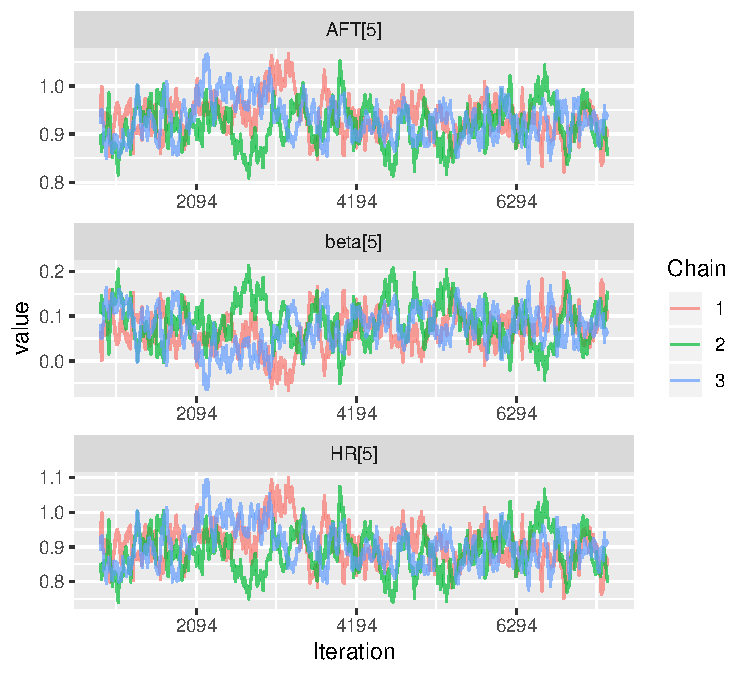
\includegraphics{HandOutEngBayes_files/figure-latex/unnamed-chunk-6-1} \caption[Traceplot for AFT, and HR of daily milk drinkers from crude model (men)]{Traceplot for AFT, and HR of daily milk drinkers from crude model (men).}\label{fig:unnamed-chunk-6}
\end{figure}
\begin{marginfigure}

{\centering 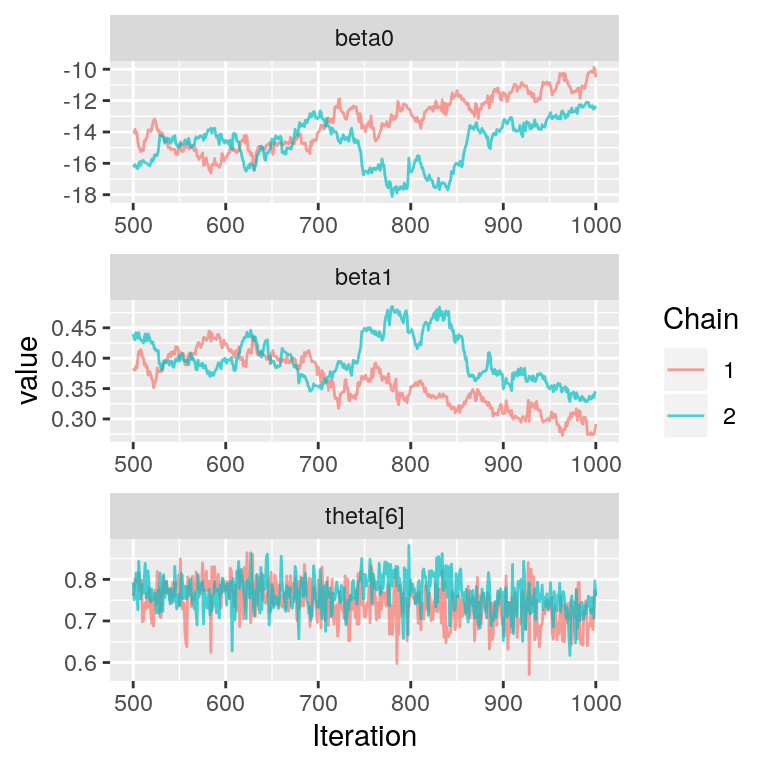
\includegraphics[width=0.9\linewidth]{fig/badtraceplot} 

}

\caption[Not overlapping traceplot indicating that model is not converged]{Not overlapping traceplot indicating that model is not converged.}\label{fig:badtrace}
\end{marginfigure}

\begin{figure}
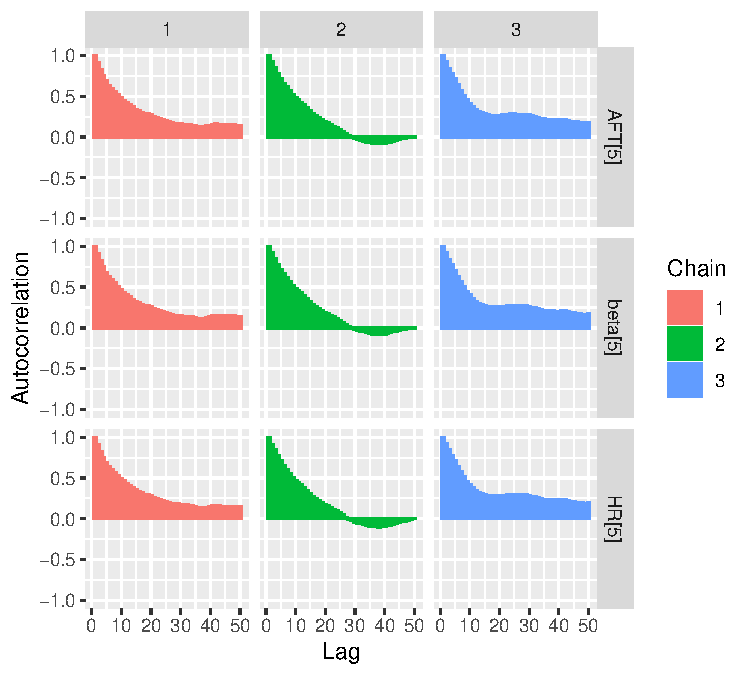
\includegraphics{HandOutEngBayes_files/figure-latex/unnamed-chunk-7-1} \caption[Autocorrelation figures for AFT, and HR of daily milk drinkers from crude model (men)]{Autocorrelation figures for AFT, and HR of daily milk drinkers from crude model (men).}\label{fig:unnamed-chunk-7}
\end{figure}

\begin{figure}

{\centering 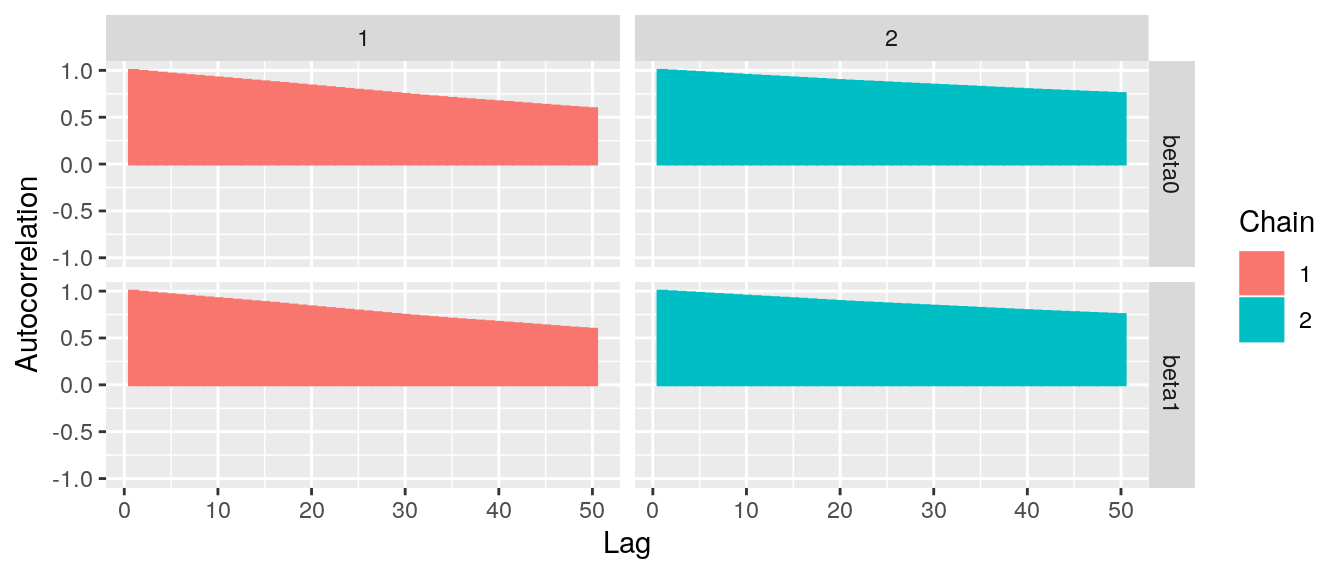
\includegraphics[width=0.9\linewidth]{fig/badautocorrelation} 

}

\caption[(bad example)Highly correlated posterior samples indicating that the samples are not independent]{(bad example)Highly correlated posterior samples indicating that the samples are not independent.}\label{fig:badauto}
\end{figure}

\begin{table}[!htbp]
Table 1. Estimated (crude) hazard ratios and acceleration factors for the association of milk intake and risk of stroke mortality using Bayesian MCMC methods in Men of the JACC study data (n = 39,386).

\centering
\fontsize{8}{10}\selectfont
\begin{tabular}[t]{llllllllll}
\toprule
\multicolumn{1}{c}{ } & \multicolumn{5}{c}{Hazard ratio (HR)} & \multicolumn{4}{c}{Acceleration factor (AF)} \\
\cmidrule(l{3pt}r{3pt}){2-6} \cmidrule(l{3pt}r{3pt}){7-10}
Milk intake & Median & Mean (SD) & 95\% CrI & MCSE & Probability & Median & Mean (SD) & 95\% CrI & MCSE\\
\midrule
\rowcolor{gray!6}  Never & - & - & - & - & - & - & - & - & -\\
1-2 t/Mon & 0.88 & 0.89 (0.09) & (0.73, 1.08) & 0.0016 & 87.15\% & 0.92 & 0.92 (0.06) & (0.81, 1.06) & 0.0011\\
\rowcolor{gray!6}  1-2 t/Week & 0.77 & 0.77 (0.07) & (0.64, 0.92) & 0.0012 & 99.63\% & 0.83 & 0.83 (0.05) & (0.74, 0.94) & 0.0009\\
3-4 t/Week & 0.79 & 0.79 (0.07) & (0.66, 0.93) & 0.0012 & 99.81\% & 0.85 & 0.85 (0.05) & (0.75, 0.95) & 0.0009\\
\rowcolor{gray!6}  Daily & 0.89 & 0.90 (0.06) & (0.79, 1.02) & 0.0010 & 95.36\% & 0.93 & 0.93 (0.04) & (0.85, 1.01) & 0.0007\\
\bottomrule
\multicolumn{10}{l}{\textit{Note: }}\\
\multicolumn{10}{l}{Abbreviations: SD, standard deviation; CrI, credible interval; MCSE, Monte Carlo Standard Error;}\\
\multicolumn{10}{l}{ Probability indicates that p for HR smaller than 1.}\\
\end{tabular}
\end{table}

\begin{figure}
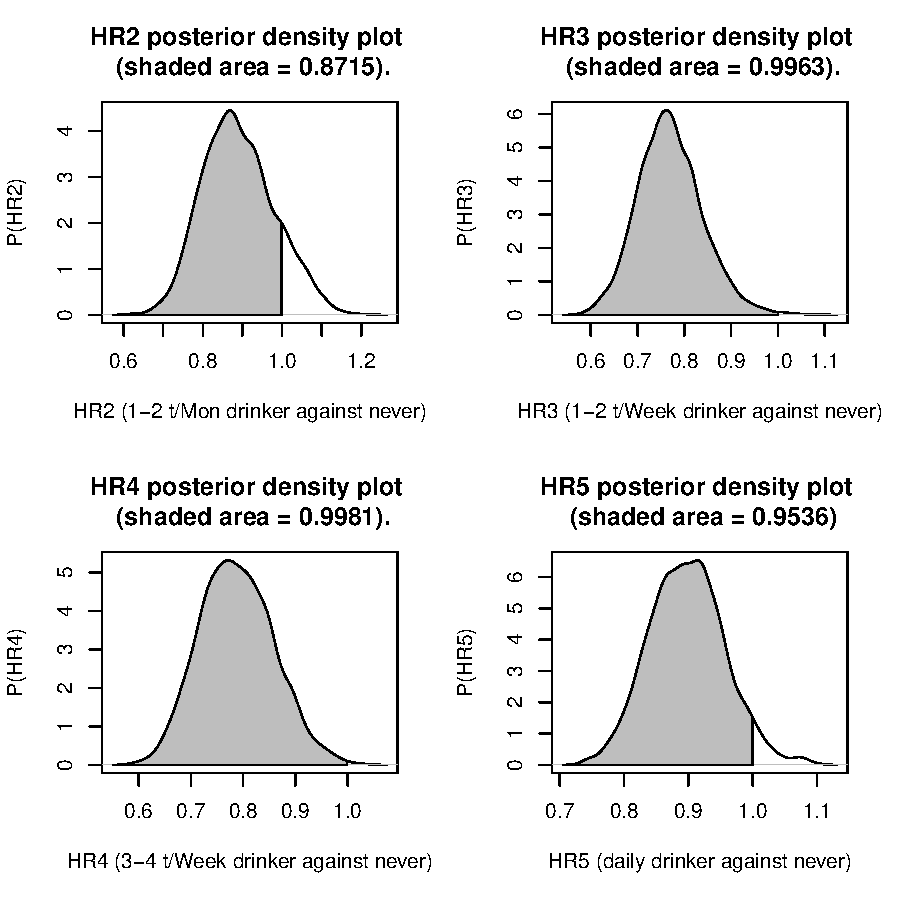
\includegraphics{HandOutEngBayes_files/figure-latex/unnamed-chunk-8-1} \caption[Crude model HR posterior density plots]{Crude model HR posterior density plots.}\label{fig:unnamed-chunk-8}
\end{figure}

\begin{table}[!htbp]
Table 2. Estimated (age-adjusted) hazard ratios and acceleration factors for the association of milk intake and risk of stroke mortality using Bayesian MCMC methods in Men of the JACC study data (n = 39,386).

\centering
\fontsize{8}{10}\selectfont
\begin{tabular}[t]{llllllllll}
\toprule
\multicolumn{1}{c}{ } & \multicolumn{5}{c}{Hazard ratio (HR)} & \multicolumn{4}{c}{Acceleration factor (AF)} \\
\cmidrule(l{3pt}r{3pt}){2-6} \cmidrule(l{3pt}r{3pt}){7-10}
Milk intake & Median & Mean (SD) & 95\% CrI & MCSE & Probability & Median & Mean (SD) & 95\% CrI & MCSE\\
\midrule
\rowcolor{gray!6}  Never & - & - & - & - & - & - & - & - & -\\
1-2 t/Mon & 0.98 & 0.98 (0.11) & (0.78, 1.19) & 0.0018 & 57.86\% & 0.98 & 0.99 (0.06) & (0.87, 1.11) & 0.0011\\
\rowcolor{gray!6}  1-2 t/Week & 0.84 & 0.84 (0.08) & (0.69, 0.99) & 0.0014 & 97.79\% & 0.90 & 0.90 (0.05) & (0.80, 0.99) & 0.0008\\
3-4 t/Week & 0.86 & 0.86 (0.08) & (0.71, 1.02) & 0.0014 & 95.92\% & 0.91 & 0.91 (0.05) & (0.82, 1.01) & 0.0009\\
\rowcolor{gray!6}  Daily & 0.75 & 0.75 (0.05) & (0.67, 0.85) & 0.0009 & 100.00\% & 0.85 & 0.85 (0.03) & (0.79, 0.91) & 0.0006\\
\bottomrule
\multicolumn{10}{l}{\textit{Note: }}\\
\multicolumn{10}{l}{Abbreviations: SD, standard deviation; CrI, credible interval; MCSE, Monte Carlo Standard Error;}\\
\multicolumn{10}{l}{ Probability indicates the p for HR smaller than 1.}\\
\end{tabular}
\end{table}

\begin{figure}
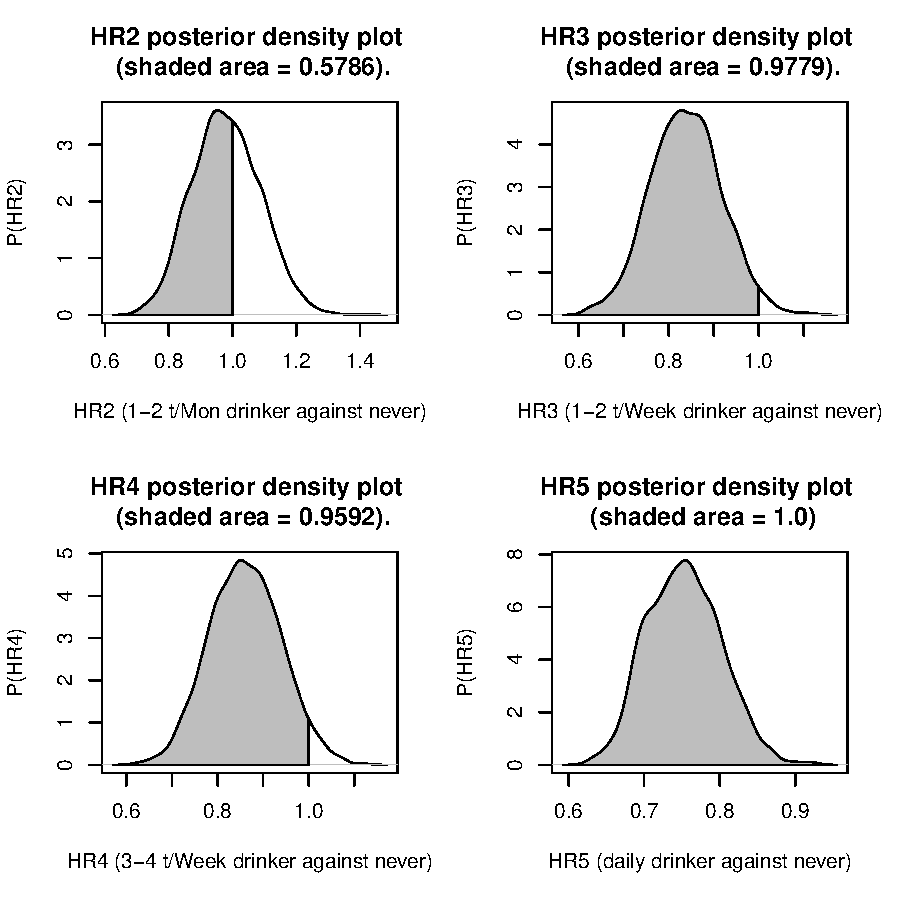
\includegraphics{HandOutEngBayes_files/figure-latex/unnamed-chunk-10-1} \caption[Age-adjusted HR posterior density plots]{Age-adjusted HR posterior density plots.}\label{fig:unnamed-chunk-10}
\end{figure}

\bibliography{skeleton.bib}



\end{document}
